\documentclass[11pt]{article}

\usepackage[margin=1in]{geometry}
\usepackage{graphicx}
\usepackage{booktabs}
\usepackage{siunitx}
\usepackage{xcolor}
\usepackage{listings}
\usepackage{caption}
\usepackage{subcaption}
\usepackage{pgfplots}
\pgfplotsset{compat=1.18}
\usepackage[colorlinks=true,linkcolor=black,urlcolor=blue]{hyperref}

% status macros so the roadmap table stays consistent as phases land
\newcommand{\done}{\textcolor{green!55!black}{\textbf{done}}}
\newcommand{\pending}{\textcolor{orange!85!black}{\textbf{pending}}}

\lstset{
  basicstyle=\ttfamily\footnotesize,
  breaklines=true,
  frame=single,
  columns=fullflexible,
  keepspaces=true,
}

\title{\textbf{CUDA-Accelerated Ray Tracer with Multi-GPU Rendering}\\[4pt]
       \large CS/EE 147 --- Spring 2026 Final Project}
\author{Chris Antony \and Kaushik Vada}
\date{Last updated: \today}

\begin{document}
\maketitle

\begin{abstract}
This is a living report for our CUDA ray tracer. The renderer loads a triangle mesh
(an OBJ exported from Fusion 360) and shades it with diffuse, metal, and dielectric
materials. We build a CPU baseline, then port it to the GPU and layer on a bounding
volume hierarchy and dual-GPU rendering, benchmarking four configurations against
each other. The document is updated phase by phase; each new configuration appends a
row to the benchmark table in Section~\ref{sec:results}. As of this revision the CPU
baseline (with mesh loading) and the naive CUDA port are complete, and the naive GPU
port is roughly three orders of magnitude faster than the single-threaded CPU on the
same scene.
\end{abstract}

\section{Overview}

The project compares four rendering configurations end to end:

\begin{enumerate}
  \item \textbf{CPU single-threaded} --- baseline, a port of Peter Shirley's
        \emph{Ray Tracing in One Weekend} extended with triangle-mesh support.
  \item \textbf{CUDA naive} --- one GPU thread per pixel, brute-force ray/scene
        intersection.
  \item \textbf{CUDA + BVH} --- a bounding volume hierarchy for sub-linear
        ray/scene intersection.
  \item \textbf{Dual-GPU} --- framebuffer split across two NVIDIA A30s.
\end{enumerate}

The end goal is a tool we can hand an arbitrary Fusion~360 export and get a rendered
image, fast enough that mesh density is not a practical limit. Configurations~3 and~4
are what make that true; configurations~1 and~2 establish the baseline and the
correctness reference.

\section{Pipeline and implementation}

\subsection{Geometry and mesh loading}

Fusion~360 exports meshes as triangle soup, so the core primitive is a single
triangle intersected with the M\"oller--Trumbore algorithm. Each triangle stores its
three vertices, an optional set of per-vertex normals, and a material index. When the
OBJ provides vertex normals (\texttt{vn}) we interpolate them across the triangle for
smooth shading; otherwise we fall back to the flat geometric normal.

The OBJ loader parses \texttt{v}, \texttt{vn}, and \texttt{f} records, handles the
\texttt{v}, \texttt{v/vt}, \texttt{v//vn}, and \texttt{v/vt/vn} face formats including
negative (relative) indices, and fan-triangulates any polygon face into $n-2$
triangles. It also returns the mesh axis-aligned bounding box, which the camera uses
to auto-frame the model: the look-at point is the box center and the camera is pulled
back along a fixed three-quarter view by a distance that fits the bounding sphere in
the vertical field of view. This means any export lands on screen regardless of its
scale or origin.

\subsection{CPU baseline}

The baseline keeps the original header-only structure (\texttt{inc/}), using
\texttt{double} precision, \texttt{std::shared\_ptr} for scene objects, and virtual
dispatch for the \texttt{hittable} and \texttt{material} hierarchies. It is
single-threaded and serves as both configuration~1 and the correctness reference for
the GPU path.

\subsection{CUDA naive port}

The GPU path is a separate type stack under \texttt{cuda/} rather than a recompile of
the CPU headers, for three reasons:

\begin{itemize}
  \item \textbf{No virtual dispatch.} Virtual functions and \texttt{shared\_ptr} do
        not translate to device code. Materials become a single plain-old-data struct
        with a type tag (lambertian / metal / dielectric); each triangle stores an
        index into a flat material array and the scatter routine switches on the tag.
  \item \textbf{Single precision.} The A30's FP64 throughput is a fraction of its
        FP32, and path tracing does not need the extra precision, so the GPU types use
        \texttt{float}.
  \item \textbf{Iterative, not recursive.} The CPU \texttt{ray\_color} recurses per
        bounce. GPU stacks are small, so the kernel folds attenuation forward in a
        bounded loop instead of recursing.
\end{itemize}

The scene (a flat triangle array plus the material array) is uploaded to device
memory once. The render kernel launches one thread per pixel on an $8\times8$ block
grid; each thread seeds a cuRAND state, accumulates \texttt{samples\_per\_pixel}
jittered samples, and writes the averaged color to the framebuffer, which is copied
back and written as a gamma-corrected PPM. Intersection in this configuration is a
brute-force linear scan over every triangle --- this is the cost the BVH in Phase~3
removes.

\section{Benchmark methodology}

\textbf{Hardware.} NVIDIA A30 (compute capability 8.0), CUDA 13.2 toolkit. CPU times
are single-threaded.

\textbf{Scene.} A UV sphere of \num{4608} triangles with per-vertex normals (smooth
shading), rendered at $800\times450$, 20 samples per pixel, maximum ray depth 10. The
same OBJ and camera framing are used for both configurations.

\textbf{What is timed.} The GPU figure is kernel time (init plus render), measured
with a host-side high-resolution clock around the launch and
\texttt{cudaDeviceSynchronize}. The CPU figure is whole-process wall-clock time; mesh
parsing for this scene is well under a tenth of a second, so the CPU number is
effectively render time.

\section{Results}
\label{sec:results}

Table~\ref{tab:bench} is the running benchmark. Rows for configurations~3 and~4 are
filled in as those phases land.

\begin{table}[h]
  \centering
  \caption{Render time on the \num{4608}-triangle sphere ($800\times450$, 20~spp,
           depth~10). Speedup is relative to the CPU baseline.}
  \label{tab:bench}
  \begin{tabular}{l S[table-format=4.2] S[table-format=4.0] l}
    \toprule
    Configuration & {Time (s)} & {Speedup ($\times$)} & Status \\
    \midrule
    CPU single-threaded & 585.23 & 1    & \done \\
    CUDA naive          & 0.47   & 1245 & \done \\
    CUDA + BVH          & {---}  & {---} & \pending \\
    Dual-GPU            & {---}  & {---} & \pending \\
    \bottomrule
  \end{tabular}
\end{table}

\begin{figure}[h]
  \centering
  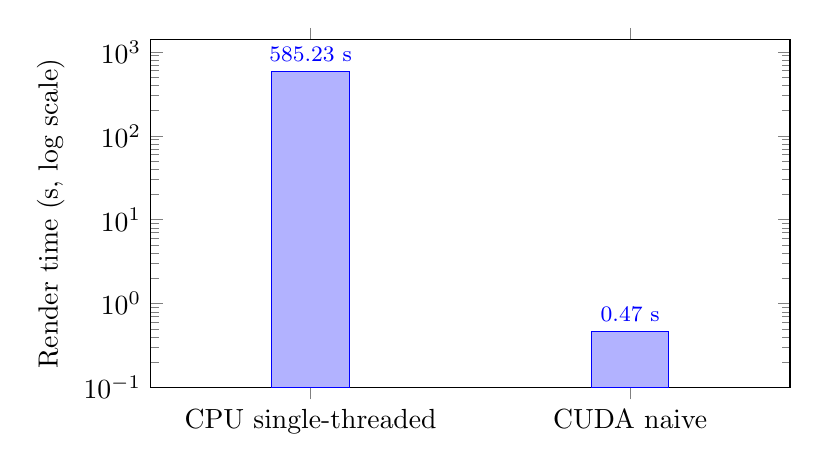
\begin{tikzpicture}
    \begin{axis}[
        width=0.8\textwidth, height=6cm,
        ybar,
        ymode=log,
        log origin=infty,
        ylabel={Render time (s, log scale)},
        symbolic x coords={CPU single-threaded, CUDA naive},
        xtick=data,
        nodes near coords,
        point meta=explicit symbolic,
        every node near coord/.append style={font=\footnotesize},
        bar width=28pt,
        ymin=0.1,
        enlarge x limits=0.5,
      ]
      % explicit labels: nodes near coords prints log-space values on a log axis otherwise
      \addplot coordinates {
        (CPU single-threaded, 585.23) [585.23 s]
        (CUDA naive, 0.47) [0.47 s]
      };
    \end{axis}
  \end{tikzpicture}
  \caption{CPU baseline vs.\ naive CUDA on the benchmark scene. Note the log axis ---
           the naive GPU port is about $1245\times$ faster.}
  \label{fig:speedup}
\end{figure}

\subsection{Correctness validation}

The GPU output is validated against the CPU baseline on the same scene. Because the
two paths use different random number generators (\texttt{std::rand} vs.\ cuRAND) and
different floating-point precision, they do not produce bit-identical images; instead
they produce the same image with independent Monte-Carlo noise. On the sphere scene
the per-channel mean absolute difference is about \num{0.2} out of \num{255}, with
isolated single-pixel maxima around \num{34} --- the signature of sampling noise, not
a geometric or shading discrepancy. Figure~\ref{fig:sphere} shows the two side by
side; Figure~\ref{fig:cube} shows the flat-shaded path on a quad-faced cube.

\begin{figure}[h]
  \centering
  \begin{subfigure}[b]{0.48\textwidth}
    \includegraphics[width=\textwidth]{figures/sphere_cpu.png}
    \caption{CPU baseline}
  \end{subfigure}
  \hfill
  \begin{subfigure}[b]{0.48\textwidth}
    \includegraphics[width=\textwidth]{figures/sphere_gpu.png}
    \caption{CUDA naive}
  \end{subfigure}
  \caption{Smooth-shaded \num{4608}-triangle sphere (interpolated vertex normals).
           CPU baseline (left) and naive CUDA (right) are visually identical; the
           only difference is independent sampling noise.}
  \label{fig:sphere}
\end{figure}

\begin{figure}[h]
  \centering
  \begin{subfigure}[b]{0.48\textwidth}
    \includegraphics[width=\textwidth]{figures/cube_cpu.png}
    \caption{CPU baseline}
  \end{subfigure}
  \hfill
  \begin{subfigure}[b]{0.48\textwidth}
    \includegraphics[width=\textwidth]{figures/cube_gpu.png}
    \caption{CUDA naive}
  \end{subfigure}
  \caption{Flat-shaded unit cube (quad faces, fan-triangulated, no vertex normals),
           exercising auto-framing and the flat-normal path.}
  \label{fig:cube}
\end{figure}

\section{Status and roadmap}

\begin{table}[h]
  \centering
  \caption{Phase status.}
  \begin{tabular}{l l l}
    \toprule
    Phase & Deliverable & Status \\
    \midrule
    1 & CPU baseline + OBJ mesh loading      & \done \\
    2 & CUDA naive port (one thread/pixel)   & \done \\
    3 & BVH acceleration                     & \pending \\
    4 & Dual-GPU rendering                   & \pending \\
    5 & Benchmarks + final writeup           & \pending \\
    \bottomrule
  \end{tabular}
\end{table}

The single most important remaining piece for the project's stated goal is the BVH
(Phase~3). Both the CPU baseline and the naive GPU port scale linearly with triangle
count, so a full-detail Fusion part is impractical until ray/scene intersection drops
to sub-linear cost. Dual-GPU (Phase~4) then splits the framebuffer across both A30s
for a further constant-factor speedup.

\section{Reproducing these numbers}

\begin{lstlisting}[language=bash]
# build (nvcc must be on PATH for the GPU target)
export PATH=/usr/local/cuda/bin:$PATH
export LD_LIBRARY_PATH=/usr/local/cuda/lib64:$LD_LIBRARY_PATH
cmake -S . -B build -DCMAKE_BUILD_TYPE=Release
cmake --build build -j

# render the benchmark scene
./build/main      sphere.obj > cpu.ppm   # config 1
./build/main_cuda sphere.obj > gpu.ppm   # config 2
\end{lstlisting}

Both binaries print timing and triangle counts to \texttt{stderr} and the PPM image
to \texttt{stdout}.

\end{document}
